


\section{Introduction}
\subsection*{Sensor theory}
Sensor fusion can be observed everywhere e.g., living animals uses all of its senses to survive daily, an animal cannot hunt using its eyes only, it has to combine its sense of smell, eyes and hearing to hunt the pray\cite{animal}. Sensor fusion theory is not only found in the living species it is found in cars, planes, computers and so on and this to enhance performance and accuracy \cite{animal}. In this project sensor fusion will be used to enhance the accuracy of the dinghy's position and velocity. The fusion will be between a global positioning system, GPS and an inertial navigation system, INS. The INS build on a low price inertial measurement unit.\\ 
The GPS's accuracy is not uniform since it might be buildings reflections, atmospherics delays or clock bias errors \cite{boken}. Using only information provided by a INS is not sufficient either since the sensors in the IMU will drift after time, but using the information provided by the sensors in the IMU only for short time will give accurate readings.  


\subsection{Kalman Filter}
A popular filter to use when applying sensor fusion is to use a Kalman filter, (KF). The Kalman Filter is a recursive filtering method for discrete data, the algorithm was developed by an Hungarian mathematician Rudolf (Rudi) Emil Kalman in 1960 \cite{boken}. Its popular to use due to its efficiency when calculating predictions. \cite{kf eff}

\subsection*{Different Frames}
Navigation algorithm involves various coordinate frames and therefore transformation between frame is a must.

The inertial frame denoted $i$-frame for future notation is defined such that its origin is at the center of Earth and its axes $X_i$, $Y_i$ and $Z_i$ is non-rotating with respect to the stars. $Z_i$ is coincident with the Earth's polar axis, i.e. North.\\

The Earth navigation frame denoted $e$-frame for future notation is fixed with respect to Earth and has its origin at the center of the Earth. The frame is defined as $X_e$, $Y_e$ and $Z_e$, with $Z_e$ along Earth's polar axis. Axis $X_e$ lies along the intersection of the plane of the Greenwich meridian with the Earth's equatorial plane. The $e$-frame rotates at a constant rate with respect to the $i$-frame and is denoted $\omega_e$.\\

The Navigation frame denoted $n$-frame for future notation is a local frame and has its origin located in the navigation system, in this case, point P, see Fig. \ref{WGS}, and its axes aligned with the directions of north, east and down, denoted NED. The turn rate of the navigation frame with respect to Earth's fixed frame, $\omega_{en}^n$, is directed by the motion of point P with respect to the Earth and is referred to the transport rate.   

\begin{figure}[H]
\centering
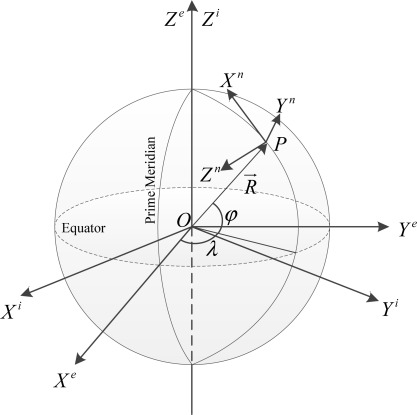
\includegraphics[width=0.3\textwidth]{Figures/WGS-coordinates.png}
\caption{Earth and navigation frame.}
\label{WGS}
\end{figure}

The Body frame denoted $b$-frame is the sensitive axes of the IMU's sensors are made to coincide with the axes of the moving platform in which the sensors are mounted. The body, in this case, is referred to the dinghy, from Fig. HÄR SKA EN BILD IN
\begin{itemize}
\item Yaw $(\psi)$: is the is the deviation of the vehicle’s forward $y$-axis from north, measured clockwise in the E-N plane.
\item Pitch $(\theta)$: This is the angle that the forward $y$-axis of the b-frame makes with the
E-N plane (i.e. local horizontal) owing to a rotation around its transversal $x$-axis.
\item Roll $(\phi)$: This is the rotation of the $b$-frame about its forward y-axis, so the
forward axis is also called the roll axis and the roll angle i
\end{itemize}

\subsection*{Transformation between Earth frame and Navigation frame}
Referring to Fig. \ref{WGS} it can be observed that its possible to align the $n$-frame with the $e$-frame, this is done by rotating the $n$-frame by ($\lambda-90$)-degrees around its $x$-axis (east-direction) and ($-\phi-90$)-degrees about its $z-axis$, (downward direction) \cite{nonlinear}. Where $\lambda$ and $\varphi$ is the latitude and longitude, respectively. Then the transformation between the two frames can be done using the Direction Cosine Matrix, noted DCM for future notation, which is defined as \cite{nonlinear}.
\begin{equation}
C_n^e=R_z(-\lambda-90)R_x(\varphi-90)
\label{Cosine_1}
\end{equation}
Where $C_n^e$ should be interpreted as moving from $n$-frame to $e$-frame, $R_x$ and $R_z$ are the rotation matrices around its axis, respectively. Expanding Eq. \eqref{Cosine_1} 
\begin{align}
C_n^e &=
\begin{bmatrix}
cos(-\lambda-90) & sin(-\lambda-90) & 0\\
-sin(-\lambda-90) & cos(-\lambda-90) & 0\\
0 & 0 & 1
\end{bmatrix}
\begin{bmatrix}
1 & 0 & 0\\
0 & cos(\varphi-90) & sin(\varphi-90) \\
0 & -sin(\varphi-90) & con(\varphi-90) \\
\end{bmatrix}\\
C_n^e &=
\begin{bmatrix}
-sin(\lambda) & -cos(\lambda) & 0\\
cos(\lambda) & -sin(\lambda) & 0\\
0 & 0 & 1
\end{bmatrix}
\begin{bmatrix}
1 & 0 & 0\\
0 & sin(\varphi) & -cos(\varphi) \\
0 & sin(\varphi) & sin(\varphi) \\
\end{bmatrix}\\
C_n^e &=
\begin{bmatrix}
-sin(\lambda) & -sin(\varphi)cos(\lambda) & cos(\varphi)cos(\lambda) \\
cos(\lambda) & -sin(\varphi)sin(\lambda) &  cos(\varphi)sin(\lambda) \\
0 & cos(\varphi) & sin(\varphi) \\
\end{bmatrix}
\end{align}
Exploring the orthogonality its possible to transform from $e$-frame to $n$-frame by taking the inverse of the equation above, i.e.
\begin{equation}
(C_n^e)^{-1}=C_e^n
\label{Eq.Earth2Nav}
\end{equation}
Using Eq. \eqref{Eq.Earth2Nav} its now possible to move from $e$-frame to $n$-frame. 


\subsection*{Transformation between Body frame and Navigation-frame}
Transforming from $n$-frame to $b$-frame is done in the same way, i.e. using rotation matrices. The DCM, moving from $b$-frame to $n$-frame is given by \cite{nonlinear}
\begin{equation}
C_b^n=R_z(-\psi)R_y(-\theta)R_x(-\phi).
\label{Body_rotation}
\end{equation}
Where 
\begin{align}
R_z(-\psi) = &
\begin{bmatrix}
cos(\psi) & -sin(\psi) & 0\\
sin(\psi) & cos(\psi) & 0 \\
0 & 0 & 1
\end{bmatrix}\label{R_z} \\
R_y(-\theta) = &
\begin{bmatrix}
cos(\theta) & 0 & sin(\theta)\\
0 & 1 & 0 \\
-sin(\theta) & 0 & cos(\theta)
\end{bmatrix}\label{R_y} \\
R_x(-\phi) = &
\begin{bmatrix}
1 & 0 & 0\\
0 & cos(\phi) & -sin(\phi)\\
0 & sin(\phi) & cos(\phi)
\end{bmatrix}\label{R_x}
\end{align}
Expanding Eq. \eqref{Body_rotation} with \eqref{R_z}, \eqref{R_y} and \eqref{R_x}
\begin{align}
C_b^n = &
\begin{bmatrix}
cos(\psi) & -sin(\psi) & 0\\
sin(\psi) & cos(\psi) & 0 \\
0 & 0 & 1
\end{bmatrix}
\begin{bmatrix}
cos(\theta) & 0 & sin(\theta)\\
0 & 1 & 0 \\
-sin(\theta) & 0 & cos(\theta)
\end{bmatrix}
\begin{bmatrix}
1 & 0 & 0\\
0 & cos(\phi) & -sin(\phi)\\
0 & sin(\phi) & cos(\phi)
\end{bmatrix}
\label{expand_Body_rotation} \\ \\
C_b^n =&
\begin{bmatrix}
cos(\theta)cos(\psi) & -cos(\phi)sin(\psi)+sin(\phi)sin(\theta)cos(\psi) &  sin(\phi)sin(\psi)+cos(\phi)sin(\theta)cos(\psi) \\
cos(\theta)sin(\psi) & cos(\phi)cos(\psi)+sin(\phi)sin(\theta)sin(\psi) & -sin(\phi)cos(\psi)+cos(\phi)sin(\theta)sin(\psi)\\
-sin(\theta) & sin(\phi)cos(\theta) & cos(\phi)cos(\theta) 
\end{bmatrix}.
\end{align}
Where $\psi$, $\theta$ and $\phi$ are the Euler angles as described earlier. \\

The angular velocity of the $e$-frame with respect to the $i$-frame projected onto the $i$-frame is given as \cite{nonlinear}
\begin{equation}
\bar{\omega}_{ie}^e = 
\begin{bmatrix}
0 & 0 & \omega_e
\end{bmatrix}^T.
\end{equation}
Where $\omega_e$ is the angular velocity of the earth in the $i$-frame and has a constant value of
$7.2921158 \times 10^{-5}$ $rad/s$ \cite{nonlinear}. Using the projection matrix Eq. \eqref{Cosine_1} its possible to project $\bar{\omega}_ {ie}^i$ onto the $n$-frame
\begin{align}
\bar{\omega}_{ie}^n=C_e^n\bar{\omega}_{ie}^e=
\begin{bmatrix}
\omega_e cos(\varphi) & 0 & -\omega_e sin(\varphi)
\end{bmatrix}^T.
\label{omega_ie}
\end{align}
$\bar{\omega}_{en}^n$ represents the turn of the $n$-frame with respect to the $e$-frame its called the transport rate and may be expressed as the rate of change of latitude and longitude as follows
\begin{align}
\bar{\omega}_{en}^n=
\begin{bmatrix}
\dot{\lambda}cos(L) & -\dot{L} & -\dot{\lambda}sin(L)
\end{bmatrix}^T.
\label{omega_en}
\end{align}
Where $\dot{\lambda}=v_e/(R_N+h)cos(L)$ and $\dot{L}=v_n/(R_E+h)$ \cite{nonlinear}, here we assume the Earth to be an ellipsoid and that there is no variation in earth gravitation depending on where the user is on the ellipsoid. $R_N$ is the meridian radius of curvature and defined as $R_N=R_0(1-e^2)/(1-e^2sin^2L)^{3/2}$ \cite{nonlinear}. $R_E$ is the transverse radius of curvature and defined as $R_E=R_0/(1-e^2sin^2L)^{1/2}$. $h$ is the height above the surface of the earth. Rewriting Eq. \eqref{omega_en} with $\dot{\lambda}$ and $\dot{L}$
\begin{align}
\bar{\omega}_{en}^n=
\begin{bmatrix}
v_e/(R_E+h) & -v_n/(R_N+h) & -v_e tan(L)/(R_N+h)
\end{bmatrix}^T \label{omega_en_ny}
\end{align}
where $v_e$ and $v_n$ are the velocities in East and North direction, respectively. Now $\bar{\omega}_{in}^n$ can be obtained by adding Eq. \eqref{omega_ie} and \eqref{omega_en_ny}.
\begin{align}
\bar{\omega}_{in}^n=
\begin{bmatrix}
\omega_e cos(\varphi) + v_e/(R_E+h) & v_n/(R_N+h) & -\omega_e sin(\varphi) + v_e tan(L)/(R_N+h)
\end{bmatrix}^T
\label{Eq.omega_in}
\end{align}

Now Eq. \eqref{Eq.omega_in} is a function dependent both on velocity and position.

\subsection*{Inertial Navigation equation}
describing the position of the dinghy in the $n$-frame is done by \cite{nonlinear}.
\begin{align}
\bar{r}^n=
\begin{bmatrix}
\varphi & \lambda & h
\end{bmatrix}^T.
\end{align}
Since velocity is described as the rate of change of its position with respect to a frame of reference, and is a function of time, the velocities in North, East and down can be expressed as.
\begin{align}
\begin{bmatrix}
v_N \\
v_E \\
v_D
\end{bmatrix}
=
\begin{bmatrix}
(R_E+h) & 0 & 0 \\
0 & (R_N+h)cos(\varphi) & 0\\
0 & 0 & -1
\end{bmatrix}
\begin{bmatrix}
\dot{\varphi}\\
\dot{\lambda}\\
\dot{h}
\end{bmatrix}
\label{Eq.v_n}
\end{align}
Where $\dot{}$ symbolizes the first derivative with respect to time. Thus, $\dot{\varphi}$, $\dot{\lambda}$ and $\dot{h}$ can be found by rewriting Eq. \eqref{Eq.v_n} as

\begin{align}
\begin{bmatrix}
\dot{\varphi}\\
\dot{\lambda}\\
\dot{h}
\end{bmatrix}
=
\begin{bmatrix}
\frac{1}{(R_E+h)} & 0 & 0 \\
0 & \frac{1}{(R_N+h)cos(\varphi)} & 0\\
0 & 0 & -1
\end{bmatrix}
\begin{bmatrix}
v_N \\
v_E \\
v_D
\end{bmatrix}
\label{Eq.v_n}
\end{align}

The velocity dynamics $\dot{\bar{v}}$ can be described in its respective direction \cite{non-linear}
\begin{equation}
\dot{v}_N = f_n-v_E(2\omega_e+\dot{\lambda})sin(L) + v_d\dot{L}+g
\label{Eq.v_n}
\end{equation}
\begin{equation}
\dot{v}_E = f_n+v_N(2\omega_e+\dot{\lambda})sin(L) + v_D(2\omega_e+\dot{\lambda})cos(L)-g
\label{Eq.v_e}
\end{equation}
\begin{equation}
\dot{v}_D = f_n-v_E(2\omega_e+\dot{\lambda})cos(L) - v_N\dot{L}+g
\end{equation}
The attitude dynamics are defined such \cite{non-linear}
\begin{equation}
\dot{C}_b^n = C_b^n\Omega_{ib}^b-\Omega_{in}^nC_b^n.
\end{equation}
The first term, $C_b^n\Omega_{ib}^b$ is a function of the body rates, as sensed by the strapdown gyroscope, the second term, $-\Omega_{in}^nC_b^n$ is a function of lower navigation frame rates. $\Omega$ is a skew matrix formed from the elements of the turn rate



\subsection*{Integration of INS/GPS Kalman Filter}
\subsubsection*{Linearizion of Non-Linear Equations}
Non-linear differential equations of navigation must be linearized in order to be usable in estimation methods such as the Kalman Filtering \cite{non-linear}. Using perturbation method to linearize the non-linearized equation for example, the perturbation of the position, velocity and attitude DCM can be expressed as:
\begin{equation}
\hat{\bar{r}}^n = \bar{r}^n + \delta\bar{r^n}
\label{Eq.pos}
\end{equation}
\begin{equation}
\hat{\bar{v}}^n = \bar{v}^n + \delta\bar{v^n}
\label{Eq.vel}
\end{equation}
\begin{equation}
\hat{C}_b^n  = (I-E^n)C_b^n
\label{eq:atti}
\end{equation}
Where $\hat{.}$ is referred to the estimated value, $\delta$ is the perturbation errors. $E^n$ is the skew-matrix of the attitude errors \cite{non-linear}, i.e.
\begin{align}
E^n=
\begin{bmatrix}
0 & -\delta_D & -\delta_E\\
\delta_D & 0 & -\delta_N \\
-\delta_E & \delta_N & 0
\end{bmatrix}
\end{align}

\subsection*{Attitude, Velocity and Position errors}
\subsubsection*{Position errors}


\subsection*{Implementing the fusion Kalman Filter}
Implementing a continuous Kalman filter using integration between Inertial Navigation System and a Global Positioning System.
\begin{align}
\hat{\bar{x}} = F \bar{x} + G \bar{u}
\label{eq.state_1}
\end{align}
Where $F$ is describing the dynamics of the system, $\bar{x}$ is the state vector, $G$ is the design matrix, $\bar{u}$ is the input matrix, i.e. forces acting on the dinghy recorded by the IMU and $\hat{\bar{x}}$ is the estimated state vector. \\

Where $F$ is a $9\times 9$ matrix and $\bar{x}$ is a $9 \times 1$ is given by
\begin{align}
F=
\begin{bmatrix}
F_{rr} & F_{rv} & 0 &\\
F_{vr} & F_{vv} & (\bar{f}^n \times)\\
F_{er} & F_{ev} & -(\bar{\omega}_{in}^n\times)
\end{bmatrix},
\qquad
\bar{x}=
\begin{bmatrix}
\delta\bar{r}^n \\
\delta\bar{v}^n\\
\delta err^n
\end{bmatrix}
\end{align}
$G$ is a $6\times6$ matrix and $\bar{u}$ is a $6 \times 1$ vector and is defined as.
\begin{align}
G=
\begin{bmatrix}
-C_b^n & 0 \\
0 & C_b^n
\end{bmatrix},
\qquad
\bar{u}=
\begin{bmatrix}
\delta \bar{\omega}_{ib}^b \\
\delta \bar{f}^b 
\end{bmatrix}
\end{align}
The elements of $\bar{u}$ is assumed to be white noise with zero mean, thus
\begin{align}
Q=diag
\begin{bmatrix}
\sigma^2_{ax} & \sigma^2_{ay} & \sigma^2_{az} & \sigma^2_{gx} & \sigma^2_{gy} & \sigma^2_{gz}
\end{bmatrix}^T
\label{Eq.Q}
\end{align}
where $\sigma^2_{a(x,y,z)}$ and $\sigma^2_{g(x,y,z)}$ is the variance for the accelerometer and gyroscope in every direction, respectively.\\

Since a computer does not use continuous time domain the equation has to be transformed into discrete domain. The state equation will then be expressed as
\begin{equation}
\hat{\bar{x}}_{k+1} = \Phi_k \bar{x}_k +  \bar{w}_k	
\label{Eq.discrete}
\end{equation}
Here $\Phi_k$ is the state transition matrix in discrete time domain, in order to  obtain a discrete state transition matrix the inverse Laplace transform is performed on the continuous state transition matrix, i.e.
\begin{equation}
\Phi_k = \mathcal{L}^{-1}\big[(SI-F)^{-1}\big]
\label{Eq.Phik}
\end{equation}
Since the sample interval, $\Delta t$ is very small in this case Eq. \eqref{Eq.Phik} can be approximated 
\begin{equation}
\Phi_k = e^{F\Delta t} \approx I + F \Delta t 
\label{Eq.Final_Phik}.
\end{equation}
From Eq. \eqref{Eq.discrete}, $\hat{w}_k$ is the driven response $t_{k+1}$ due to the input white noise. White noise is uncorrelated between sample periods, i.e the noise between $t_k$ and $t_{k+1}$ is uncorrelated \cite{signal_process}. Then the covariance matrix which is associated with $\bar{w}_k$ is \cite{signal_process}

\begin{align}
\mathbb{E}[\bar{w_i}\bar{w}_j^T] =
\begin{cases}
  Q_k &\quad i=j\\    
  0 &\quad i\neq j   
\end{cases}
\end{align}

and $Q_k$ can then be approximated using first order of the discrete transition matrix \cite{Discrete_kalman}
\begin{equation}
Q_k\approx \Phi_k GQG^T \Phi_k^T.
\label{Eq.Q_k}
\end{equation}

If Eq. \eqref{Eq.Q} is analyzed, by increase the norm of $Q_k$ the Kalman filter trusts the measurements more than the system, which will make the output more noisy due to noise induced from the measurements, the advantages with a large norm is that the time lag will decrease. If the norm is small the measurements will be less induced with measurement noise but time lag will increase, which means that we don't trust the measurements. Determining $Q_k$ can be done by testing several different settings and from that make an assumption, but a good assumption should be that the trajectory of the output should follow the GPS data.\\



The Kalman filter is a linear quadratic estimator which is recursive and the estimator is unbiased and has minimum variance. the algorithm starts from a random process model, i.e. Eq. \eqref{Eq.discrete} and the following observation matrices \cite{Discrete_kalman}.

\begin{equation}
z_k = H_k\bar{x}_k + \bar{e}_k
\end{equation}
where $z_k$ is the measurement vector and $e_k$ is random measurement noise, with following characteristics \cite{signal_process}.
\begin{align}
\mathbb{E}[\bar{e_i}\bar{e}_j^T] =
\begin{cases}
  R_k &\quad i=j\\    
  0 &\quad i\neq j   
\end{cases}
\end{align}

The Kalman Filter can be seen as a two step filter with a prediction update and a correction update. In the latter case the Kalman gain is first calculated by
\begin{equation}
K_k = P_k^-H^T(HP_k^-H^T+R_k)^{-1}
\end{equation}
then the state vector is updated
\begin{equation}
\hat{x}_k = \hat{x}_k^- + K_k(z_k-H\hat{x}_k^-)
\end{equation}
the last step is updating the covariance matrix
\begin{equation}
P_k = (I-K_kH)P_k^-
\end{equation}

When correction update is done the algorithm makes a prediction update this is done by 
\begin{equation}
\hat{x}_k^- = \hat{\bar{x}}_k\Phi_k
\end{equation}
then updating its covariance
\begin{equation}
P_k^- = \Phi_k P_k \Phi_k^T + Q_k^.
\end{equation}
Where $(._k^-)$ should be interpreted such as calculating the prediction at time $k$ given time $k-1$.\\

The measurement vector $z_k$ is containing the difference of velocity and position from the INS and GPS
\begin{align}
z_k =
\begin{bmatrix}
\lambda_{INS} - \lambda_{GPS} \\
\varphi_{INS} - \varphi_{GPS} \\
h_{INS} - h_{GPS} \\
v_{nINS} - v_{nGPS} \\
v_{eINS} - v_{eGPS} \\
v_{hINS} - v_{hGPS}
\end{bmatrix}
\end{align}
The measurement matrix $H_k$ is defined such
\begin{align}
H_k = 
\begin{bmatrix}
I_{3\times 3} && 0_{3 \times 3} && 0_{3 \times 3} \\
0_{3 \times 3} && I_{3\times 3} && 0_{3 \times 3}
\end{bmatrix}
\end{align}

The measurement noise matrix $R_k$ is defined such as 
\begin{equation}
R_k = diag(\sigma_{r_n}^2 \quad \sigma_{r_e}^2 \quad \sigma_{r_d}^2 \quad \sigma_{v_n}^2 \quad \sigma_{v_e}^2 \quad \sigma_{v_d}^2)
\end{equation}
where $\sigma_{r}^2$ and $\sigma_{v}^2$ is the variance of the position and velocity in all direction, respectively.\\

The Kalman Filter is invoked every time the GPS is updated, i.e. $1Hz$, but since the IMU and the GPS updates at different frequencies a problem arises. The problem is such that at $t_{GPS}(k)$ there won't be a value to read from the IMU, since discrete time domain. To solve this problem a linear interpolation is done between $t_{imu}(k)$ and $t_{imu}(k+1)$, where $t_{imu}(k)$ $\leq$ $t_{GPS}(k)$ $\geq$  $t_{imu}(k+1)$. See Fig. \ref{Fig.different_update}.
\begin{figure}[H]
\centering
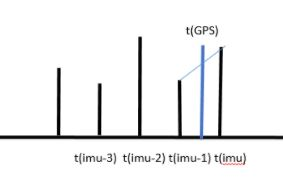
\includegraphics[width=0.4\textwidth]{Figures/linear.JPG}
\caption{Different update sequences IMU and GPS}
\label{Fig.different_update}
\end{figure}

The following linear interpolation equation is used for calculating the positions at $t_{GPS}(k)$
\begin{equation}
r_n(t_k(GPS) = r_n(t_{imu}(k)) + \frac{r_n(t_{imu}(k+1))-r_n(t_{imu}(k))}{t_{imu}(k+1)-t_{imu}(k)}(t_{GPS}(k)-t_{GPS}(k))
\end{equation}
 and the equations for the velocities 
 \begin{equation}
v_n(t_k(GPS) = v_n(t_{imu}(k)) + \frac{v_n(t_{imu}(k+1))-v_n(t_{imu}(k))}{t_{imu}(k+1)-t_{imu}(k)}(t_{GPS}(k)-t_{GPS}(k)).
\end{equation}


























